Nessa seção, que encerra o capítulo, é exibido um resumo dos resultados apresentados no decorrer do mesmo. Em seguida, uma análise geral dos métodos avaliados é empregada, destacando-se as principais qualidades e deficiências associadas a cada um dos pacotes utilizados. Por fim, é introduzida uma metodologia que possibilita a suavização das trajetórias de controle associadas a um estudo de caso qualquer. 

\subsection{Síntese dos resultados obtidos}
\label{sec:resultados:conclusao:resumo}
\todo[inline, color=pink, size=normalsize]{Relação entre $ t_p $ e $ n_{aval} $}

Tendo em vista os resultados apresentados no decorrer desse capítulo, vale ressaltar primeiramente que nem sempre verifica-se uma relação direta entre $ t_p $ e $ n_{aval} $. É possível que os $ t_p $ mais baixos, estejam associados aos $ n_{aval} $ mais altos, por mais que isso pareça ser contraintuitivo. Esse comportamento pode ser verificado quando avaliam-se os resultados apresentados nas Tabelas \ref{tab:integrador:raw}-\ref{tab:foguete:raw}, principalmente aqueles associados ao $ PSOPT $. De fato, o aumento de $ n_{aval} $ promove o crescimento de $ t_p $, no entanto, verifica-se que $ t_p $ é mais sensível ao aumento de $ N $ do que ao de $ n_{aval} $.

\todo[inline, color=pink, size=normalsize]{Relação entre $ N $ e $ t_p $ e entre $ N $ e $ n_{aval} $}

Além disso, sabe-se que $ n_{aval} $ depende fortemente do tipo de colocação utilizado \cite{kelly_introduction_2017}. Diante disso, é possível que um alto $ N $ possa estar associado a um baixo $ n_{aval} $, ou vice-versa, como ocorre nas Tabelas \ref{tab:singular2:raw}, \ref{tab:penduloInvertido:raw}, \ref{tab:uav:raw}, e \ref{tab:foguete:raw}. Esses resultados indicam que é preciso cautela na comparação de métodos baseados em diferentes tipos de colocação. 

\todo[inline, color=pink, size=normalsize]{Comparação entre as colocações trapezoidal, Hemite-Simpson e pseudo-espectral (usando $ PSOPT $)}

Quando comparam-se os resultados obtidos por meio do $ PSOPT_t $, do $ PSOPT_h $ e do $ PSOPT_l $, verifica-se que são comumente atribuídos à colocação pseudo-espectral $ N_m $ menores que aqueles associados aos demais métodos. São exceções os estudos de caso introduzidos na Seção \ref{sec:resultados:singulares}, uma vez que o $ PSOPT $ não apresenta um bom desempenho na resolução de problemas singulares, e na Seção \ref{sec:resultados:uav}, considerando-se que, nesse caso, foi necessário aumentar drasticamente o $ N_m $ associado ao $ PSOPT_l $ devido ao aparecimento de um distúrbio numérico em um dos controles. 

Tais observações podem ser verificadas por meio da análise da Figura \ref{fig:resultados:conclusao:NPSOPTthl}. Para que o gráfico de barras apresentado nessa figura seja construído, são atribuídos pontos a cada um dos métodos em análise, com base nos $ N_m $ associados aos mesmos. Um ponto é atribuído a um dado método quando associa-se ao mesmo o menor dos $ N_m $ obtidos na resolução de um dado estudo de caso. Acima de cada barra é mostrada a somatória dos pontos atribuídos a cada método, enquanto na legenda do gráfico estão listados os estudos de caso a partir dos quais esses pontos foram obtidos. Caso $ N_m $ iguais estejam associados a métodos diferentes, é possível que haja um empate, e nesse caso, um ponto é concedido a cada método. Caso ocorra um empate, é possível que um dado estudo de caso seja listado duas vezes na legenda. Vale ressaltar que outros gráficos semelhantes àquele introduzido na Figura \ref{fig:resultados:conclusao:NPSOPTthl} são apresentados no decorrer dessa seção. Tais gráficos seguem a mesma lógica de atribuição de pontos, mas têm como base a análise de outras métricas, como o tempo de execução ou o número de avaliações da função objetivo. No título de cada gráfico é indicada a métrica na qual baseia-se a construção do mesmo.

De fato, avaliando-se o gráfico apresentado na Figura \ref{fig:resultados:conclusao:NPSOPTthl}, é possível comprovar que os menores $ N_m $ são comumente atribuídos ao $ PSOPT_l $, com exceção dos estudos de caso introduzidos nas Seções \ref{sec:resultados:singulares} e \ref{sec:resultados:uav}.

\noindent	
\begin{minipage}{\textwidth}
	\vspace{\onelineskip}
	\centering
	\includegraphics[width=1\linewidth]{fig/resultados/ranking/3/N}
	\captionof{figure}[Avaliação do número de nós de colocação atribuídos ao $ PSOPT_t $, ao $ PSOPT_h $ e ao $ PSOPT_l $]{Avaliação dos $ N_m $ atribuídos ao $ PSOPT_t $, ao $ PSOPT_h $ e ao $ PSOPT_l $.}
	\label{fig:resultados:conclusao:NPSOPTthl}
	\vspace{\onelineskip}
\end{minipage}

Como consequência das diferenças entre os $ N_m $ associados a cada tipo de colocação, verifica-se que, no geral, atribuem-se ao $ PSOPT_l $ e ao $ PSOPT_h $ $ t_p $ menores que os atribuídos ao $ PSOPT_t $, como indica o gráfico apresentado na Figura \ref{fig:resultados:conclusao:tpPSOPTthl}. 

\noindent	
\begin{minipage}{\textwidth}
	\vspace{\onelineskip}
	\centering
	\includegraphics[width=1\linewidth]{fig/resultados/ranking/3/t}
	\captionof{figure}[Avaliação dos tempos de processamento atribuídos ao $ PSOPT_t $, ao $ PSOPT_h $ e ao $ PSOPT_l $]{Avaliação dos $ t_p $ atribuídos ao $ PSOPT_t $, ao $ PSOPT_h $ e ao $ PSOPT_l $.}
	\label{fig:resultados:conclusao:tpPSOPTthl}
	\vspace{\onelineskip}
\end{minipage}

Além disso, estão associados ao $ PSOPT_l $ $ n_{aval} $ menores que os atribuídos ao $ PSOPT_t $ e ao $ PSOPT_h $, como indica o gráfico da Figura \ref{fig:resultados:conclusao:navalPSOPTthl}. Essa máxima vale para a maioria dos estudos de caso monofásicos, com exceção daquele introduzido na Seção \ref{sec:resultados:uav}, no qual verificou-se o distúrbio numérico citado anteriormente. Vale ressaltar que, avaliando-se os resultados introduzidos na Seção \ref{sec:resultados:singulares}, verifica-se que é atribuído ao $ PSOPT_l $ um $ n_{aval} $ menor que os associados ao $ PSOPT_t $ e ao $ PSOPT_h $, ainda que os $ N_m $ atribuídos aos mesmos sejam consideravelmente menores que aquele associado ao $ PSOPT_l $.

\noindent	
\begin{minipage}{\textwidth}
	\vspace{\onelineskip}
	\centering
	\includegraphics[width=1\linewidth]{fig/resultados/ranking/3/eval}
	\captionof{figure}[Análise do número de avaliações da função objetivo atribuídos ao $ PSOPT_t $, ao $ PSOPT_h $ e ao $ PSOPT_l $]{Avaliação dos $ n_{aval} $ atribuídos ao $ PSOPT_t $, ao $ PSOPT_h $ e ao $ PSOPT_l $.}
	\label{fig:resultados:conclusao:navalPSOPTthl}
	\vspace{\onelineskip}
\end{minipage}

Comparando-se ainda as soluções obtidos por meio do $ PSOPT_t $, do $ PSOPT_h $, do $ COPILOTS_t $, e do $ COPILOTS_h $, observa-se que os $ N_m $ associados à colocação Hermite-Simpson são tipicamente menores que aqueles atribuídos à colocação trapezoidal, como indicam os gráficos apresentados nas Figuras \ref{fig:resultados:conclusao:NthCOPILOTS} e \ref{fig:resultados:conclusao:NthPSOPT}. Esses resultados se devem às propriedades numéricas inerentes a cada tipo de colocação e dos métodos empregados na interpolação dos estados e controles.

\noindent	
\begin{minipage}{\textwidth}
	\vspace{\onelineskip}
	\centering
	\includegraphics[width=1\linewidth]{fig/resultados/ranking/2/N}
	\captionof{figure}[Avaliação do número de nós de colocação atribuídos ao $ COPILOTS_t $ e ao $ COPILOTS_h $]{Avaliação dos $ N_m $ atribuídos ao $ COPILOTS_t $ e ao $ COPILOTS_h $.}
	\label{fig:resultados:conclusao:NthCOPILOTS}
	\vspace{\onelineskip}
\end{minipage}

\noindent	
\begin{minipage}{\textwidth}
	\vspace{\onelineskip}
	\centering
	\includegraphics[width=1\linewidth]{fig/resultados/ranking/1/N}
	\captionof{figure}[Avaliação do número de nós de colocação atribuídos ao $ PSOPT_t $ e ao $ PSOPT_h $]{Avaliação dos $ N_m $ atribuídos ao $ PSOPT_t $ e ao $ PSOPT_h $.}
	\label{fig:resultados:conclusao:NthPSOPT}
	\vspace{\onelineskip}
\end{minipage}

\todo[inline, color=pink, size=normalsize]{Problemas singulares no $ PSOPT $}

Como esperado, verifica-se que o emprego da colocação pseudo-espectral na solução de PCOs singulares não traz resultados satisfatórios \cite{becerra_tutorial_2010}. De fato, nas soluções atribuídas ao $ PSOPT_l $, introduzidas na Seção \ref{sec:resultados:singulares}, observam-se $ N_m $ bastante altos e trajetórias de controle consideravelmente oscilatórias. Resultados mais aceitáveis poderiam ser obtidos caso os PCOs singulares fossem formulados empregando-se múltiplas fases \cite{nascentes_resolucao_2012}. Uma outra alternativa seria empregar a abordagem introduzida na Seção \ref{sec:resultados:conclusao:suavizacaoTrajetorias}, que possibilita a obtenção de trajetórias mais suaves.

\todo[inline, color=pink, size=normalsize]{Limitação do Método de Ponto Interior do $ PSOPT $}

Além disso, verifica-se que o Método de Ponto Interior no qual se baseia o IPOPT \cite{wachter_implementation_2006}, pacote utilizado pelo $ PSOPT $ na solução de PPNLs, não apresenta um bom desempenho quando empregado na resolução de PCOs que contenham muitas restrições em sua formulação. De fato, avaliando-se os resultados apresentados na Tabela \ref{tab:estacionamento:raw}, nota-se que são atribuídos ao $ PSOPT $ $ N_s\% $ consideravelmente baixos. 

\todo[inline, color=pink, size=normalsize]{Trajetórias do $ PSOPT_l $}

Verifica-se que as trajetórias construídas com base nos resultados advindos da colocação pseudo-espectral são consideravelmente mais suaves que aquelas produzidas por meio de outros tipos de colocação. Esse comportamento se deve ao fato das trajetórias associadas à colocação pseudo-espectral serem interpoladas globalmente, empregando-se um único polinômio de alta ordem \cite{becerra_psopt_2019}. 

\todo[inline, color=pink, size=normalsize]{Reconstrução da trajetória do $ PSOPT_h $:}

É essencial frisar que os dados fornecidos pelo $ PSOPT_h $, após a resolução de um estudo de caso qualquer, são insuficientes para que construam-se as trajetórias de controle. Isso porque a interpolação de trajetórias na qual se baseia a colocação Hermite-Simpson depende não só dos valores que $ \mathbf{u}(t) $ assume nos nós de colocação, mas também dos valores assumidos por $ \mathbf{u}(t) $ nos nós intermediários, que não são fornecidos pelo $ PSOPT $. 

\todo[inline, color=pink, size=normalsize]{Qualidades do $ FALCON $}

Verifica-se que na maioria dos casos são atribuídos ao $ FALCON $ os menores $ t_p $ e $ n_{aval} $, como indicam os gráficos nas Figuras \ref{fig:resultados:conclusao:tpFALCON} e \ref{fig:resultados:conclusao:navalFALCON}. Além disso, normalmente estão associados a esse pacote $ N_s\% $ bem próximos a 100\%. Esses resultados podem ser justificados por dois principais fatores. Primeiro, ao uso que o $ FALCON $ faz de ferramentas simbólicas na obtenção das derivadas analíticas da função objetivo e das restrições, e segundo, à geração e ao emprego de arquivos de extensão \texttt{.mex}, que convertem, de forma automática, os códigos em Matlab\textsuperscript{\textregistered} utilizados na formulação do PCO em rotinas baseadas em linguagens de baixo nível como C/C++ e Fortran. De fato, é sabido que o emprego de derivadas analíticas acarreta uma diminuição no número de avaliações da função objetivo e consequentemente no tempo de processamento \cite{betts_practical_2001}. Além disso, o emprego de linguagens de baixo nível pré-compiladas proporciona uma redução ainda maior no tempo de processamento \cite{febbo_nloptcontrol_2020}. 

\noindent	
\begin{minipage}{\textwidth}
	\vspace{\onelineskip}
	\centering
	\includegraphics[width=1\linewidth]{fig/resultados/ranking/all/t}
	\captionof{figure}[Avaliação dos tempos de processamento atribuídos a todos os pacotes avaliados]{Avaliação dos $t_p$ atribuídos a todos os pacotes avaliados.}
	\label{fig:resultados:conclusao:tpFALCON}
	\vspace{\onelineskip}
\end{minipage}

\noindent	
\begin{minipage}{\textwidth}
	\vspace{\onelineskip}
	\centering
	\includegraphics[width=1\linewidth]{fig/resultados/ranking/all/eval}
	\captionof{figure}[Análise do número de avaliações da função objetivo atribuídas a todos os pacotes avaliados]{Avaliação dos $ n_{aval} $ atribuídos a todos os pacotes avaliados.}
	\label{fig:resultados:conclusao:navalFALCON}
	\vspace{\onelineskip}
\end{minipage}

Destaca-se que o único estudo de caso, formulado com base em uma única fase, no qual não é atribuído ao $ FALCON $ o menor $ t_p $, é aquele apresentado na Seção \ref{sec:resultados:uav}. Esse resultado indica que e pacote tem, de fato, como principal vantagem a computação de derivadas analíticas, recurso que não pode ser empregado no estudo de caso em questão, uma vez que a dinâmica associada ao mesmo depende da interpolação linear dos dados de uma tabela. 

\todo[inline, color=pink, size=normalsize]{$ FALCON $ e o impacto de $ N $}

Além do mais, verifica-se que os $ t_p $ e $ n_{aval} $ associados ao $ FALCON $ são praticamente insensíveis ao aumento de $ N $, devido ao uso que esse pacote faz de ferramentas simbólicas na computação de derivadas analíticas. Nas Figuras \ref{fig:resultados:conclusao:Nxt} e \ref{fig:resultados:conclusao:Nxn}, que têm o eixo das abcissas em escala logarítmica, são comparados os $ t_p $ e $ n_{aval} $ associados à resolução do estudo de caso introduzido na Seção \ref{sec:resultados:penduloInvertido}, empregando-se o $ PSOPT_t $ e o $ FALCON $, e considerando-se $ N $ razoavelmente altos. Por meio da avaliação desses resultados, é possível verificar primeiramente que, para $ N $ pequenos, o $ FALCON $ executa tão rapidamente quando o $ PSOPT_t $, que é baseado nas linguagens C/C++, e que os $ t_p $ associados ao primeiro, diferentemente daqueles atribuídos ao segundo, são muito pouco sensíveis ao aumento de $ N $. 

Vale ressaltar, no entanto, que essa diferença nos $ t_p $ associados ao $ FALCON $ e ao $ PSOPT $ se devem principalmente ao cálculo do erro de discretização das equações diferenciais associadas à dinâmica do PCO, computado pelo $ PSOPT $ mas não pelo $ FALCON $. O tempo gasto no processamento desse erro aumenta consideravelmente à medida que $ N $ cresce, enquanto o tempo despendido de fato na solução do PPNL não apresenta um crescimento considerável à medida que $ N $ aumenta.  

Além disso, é possível verificar que os $ n_{aval} $ associados ao $ FALCON $ são significativamente menores que os atribuídos ao $ PSOPT_t $, e praticamente insensíveis ao aumento de $ N $. Esse resultado se deve ao uso que o $ FALCON $ faz das derivadas analíticas da função objetivo e das restrições. 

\noindent	
\begin{minipage}{\textwidth}
	\vspace{\onelineskip}
	\centering
	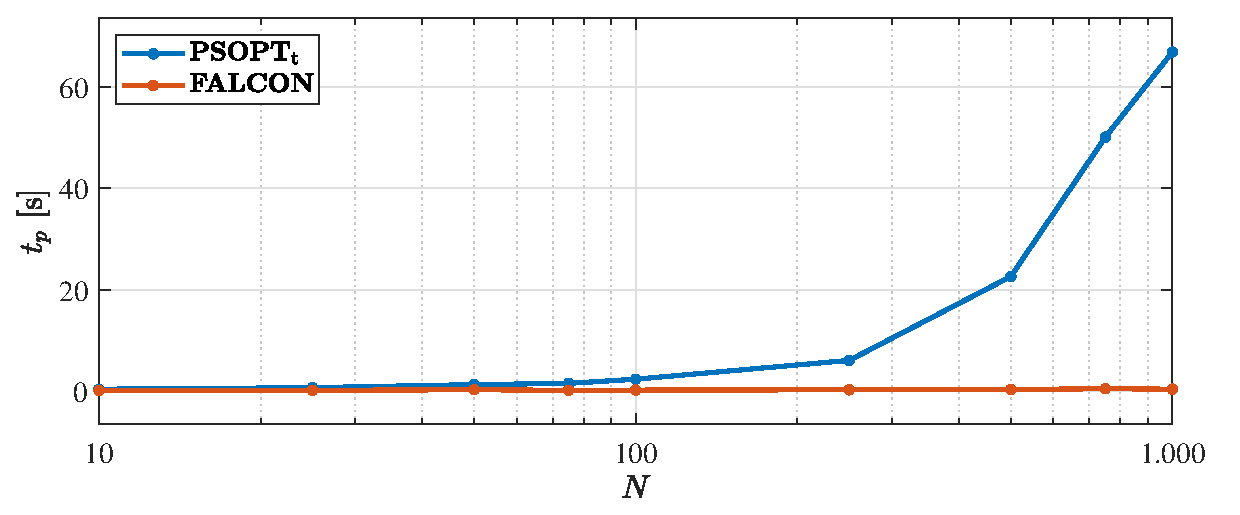
\includegraphics[width=1\linewidth]{fig/resultados/obs/bigN/Nxt}
	\captionof{figure}[Avaliação dos tempos de processamentos atribuídos ao $ PSOPT_t $ e o $ FALCON $, para o problema do pêndulo invertido, considerando-se um número de nós de colocação razoavelmente alto]{Comparação entre os $ t_p $ associados à resolução do estudo de caso apresentado na Seção \ref{sec:resultados:penduloInvertido} empregando-se o $ PSOPT_t $ e o $ FALCON $, e considerando-se $ N $ razoavelmente altos.}
	\label{fig:resultados:conclusao:Nxt}
	\vspace{\onelineskip}
\end{minipage}

\noindent	
\begin{minipage}{\textwidth}
	\vspace{\onelineskip}
	\centering
	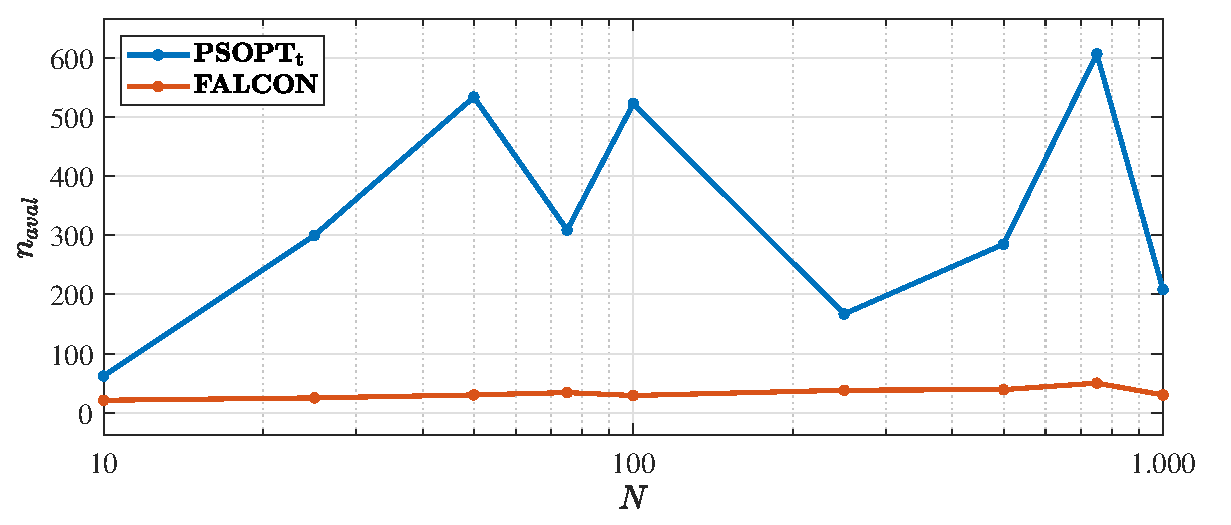
\includegraphics[width=1\linewidth]{fig/resultados/obs/bigN/Nxn}
	\captionof{figure}[Análise das avaliações da função objetivo atribuídas ao $ PSOPT_t $ e o $ FALCON $, para o problema do pêndulo invertido, considerando-se um número de nós de colocação razoavelmente alto]{Comparação entre os $ n_{aval} $ associados à resolução do estudo de caso apresentado na Seção \ref{sec:resultados:penduloInvertido} empregando-se o $ PSOPT_t $ e o $ FALCON $, e considerando-se $ N $ razoavelmente altos.}
	\label{fig:resultados:conclusao:Nxn}
	\vspace{\onelineskip}
\end{minipage}

\todo[inline, color=pink, size=normalsize]{$ FALCON $ e os multifásicos}

Apesar dos bons resultados obtidos por meio do $ FALCON $, é preciso ressaltar que o estudo de caso introduzido na Seção \ref{sec:resultados:foguete} não pode ser resolvido pelo emprego desse pacote, já que, nesse caso, o processo de otimização atinge um mínimo local que não atende às restrições do problema e ali permanece. O PCO associado a esse estudo de caso possui múltiplas fases e, apesar do $ FALCON $ ser capaz de resolver problemas desse tipo, não é apresentada na documentação associada a esse pacote qualquer exemplo de um problema multifásico que tenha dinâmicas distintas associadas a cada fase, como é o caso do PCO em questão. 

\todo[inline, color=pink, size=normalsize]{Observações sobre o $ COPILOTS $}

Verifica-se que ao $ COPILOTS $ estão comumente atribuídos os menores $ J^* $, como indica o gráfico na Figura \ref{fig:resultados:conclusao:JCOPILOTS}, e os maiores $ N_s\% $, devido ao uso que o pacote faz do SQP. Em contrapartida, ao $ COPILOTS $ estão também associados os maiores $ t_p $ e $ n_{aval} $, não só pelo emprego do $ SQP $, mas também devido ao uso que o $ COPILOTS $ faz da função \texttt{fmincon()}, nativa do Matlab\textsuperscript{\textregistered}, na solução de PPNLs, algo que é fortemente desaconselhado pelos desenvolvedores de outros pacotes \cite{falugi_iclocs2_2018}. O uso dessa função pode inclusive explicar os baixíssimos $ N_s\% $ atribuídos ao $ COPILOTS $ na resolução dos estudos de caso introduzidos nas Seções \ref{sec:resultados:estacionamento}, que apresenta um número consideravelmente alto de restrições, e \ref{sec:resultados:uav}, que possui uma dinâmica descontínua que depende da interpolação linear dos dados de uma tabela. Além disso, verifica-se que os menores $ J^* $ são atribuídos aos métodos que fazem uso da colocação Hermite-Simpson, devido às propriedades numéricas associadas a esse tipo de colocação, que faz uso de nós intermediários na interpolação dos estados e controles. 

\noindent	
\begin{minipage}{\textwidth}
	\vspace{\onelineskip}
	\centering
	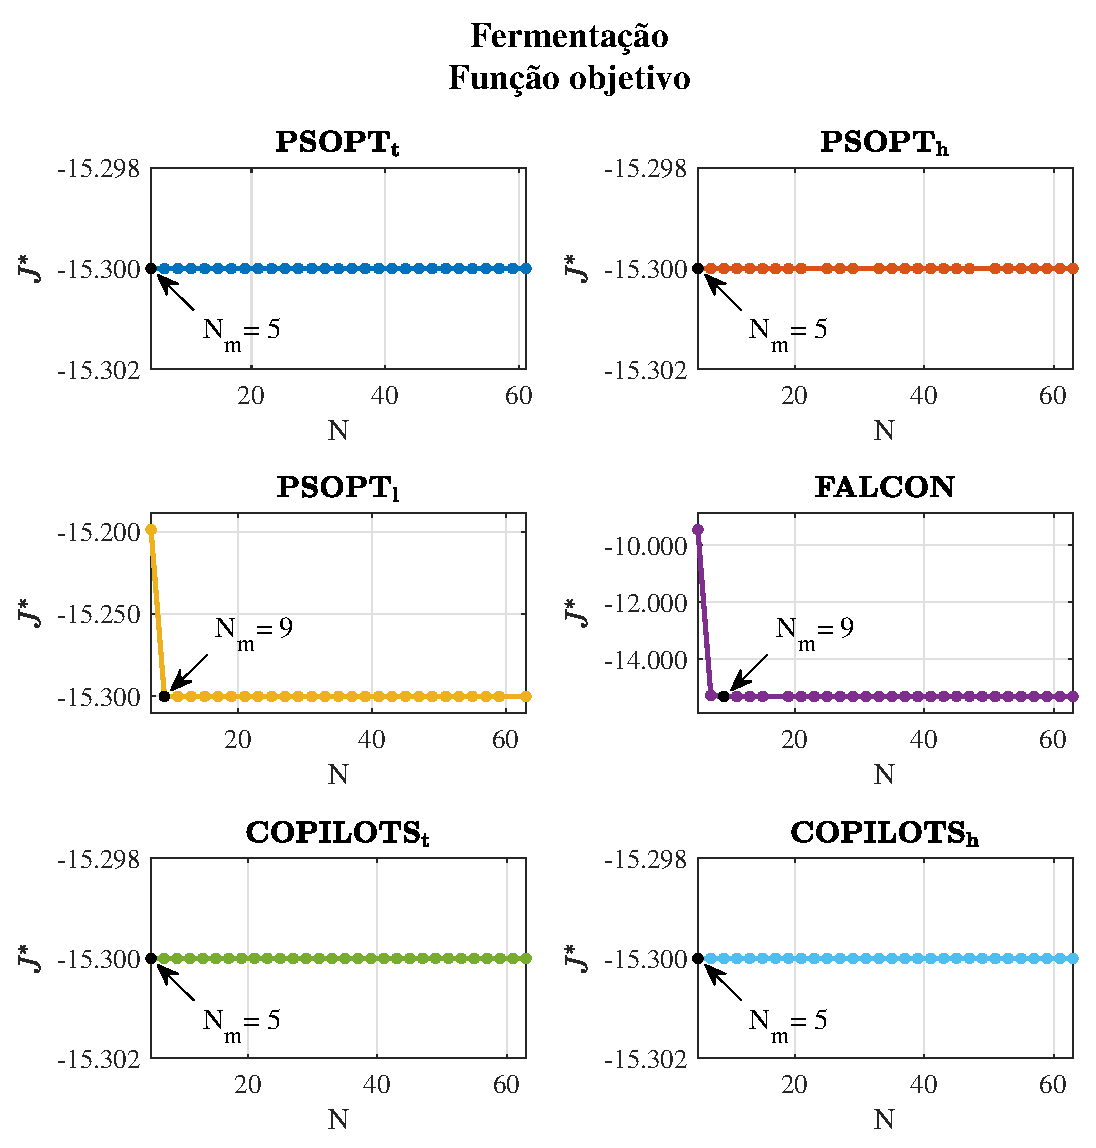
\includegraphics[width=1\linewidth]{fig/resultados/ranking/all/J}
	\captionof{figure}[Avaliação dos valores ótimos da função objetivo atribuídos a todos os pacotes avaliados]{Avaliação dos $ J^* $ atribuídos a todos os pacotes avaliados.}
	\label{fig:resultados:conclusao:JCOPILOTS}
	\vspace{\onelineskip}
\end{minipage}

\todo[inline, color=pink, size=normalsize]{Resumo}

Os resultados obtidos podem ser resumidos da seguinte forma:
\begin{itemize}
	\item Recomenda-se o emprego do $ PSOPT $ na resolução de PCOs multifásicos;
	\item Não é recomendado que a colocação pseudo-espectral seja empregada na resolução de PCOs singulares;
	\item No caso em que a minimização da função objetivo é especialmente relevante e que o tempo de execução, assim como o número de avaliações da função objetivo, são pouco importantes, recomenda-se que o $ COPILOTS $ seja utilizado juntamente à colocação Hermite-Simpson;
	\item Caso o usuário tenha pouca ou nenhuma experiência com a implementação computacional de PCOs, ou caso tenha o intuito empregar um pacote computacional para fins didáticos, recomenda-se a utilização do $ COPILOTS $;
	\item Caso seja necessário resolver um PCO empregando o mínimo de avaliações da função objetivo no menor tempo possível, recomenda-se o emprego do $ FALCON $;
	\item Não é recomendado que o $ FALCON $ seja utilizado na resolução de PCOs multifásicos que possuam uma dinâmica distinta associada a cada fase;
\end{itemize}

\subsection{Análise geral dos pacotes avaliados}
\label{sec:resultados:conclusao:analiseGeral}
Nessa seção são apresentadas algumas questões que devem ser respondidas pelo usuário que pretende escolher o pacote mais adequado. Alguns comentários acerca dos métodos avaliados no presente trabalho são elaborados, porém, é necessário que se tenha em mente que as questões aqui apresentadas podem servir de base para comparação de pacotes que não foram aqui avaliados, ou mesmo que não tenham sido desenvolvidos para resolução de PCOs \cite{parejo_metaheuristic_2012}. 

\begin{itemize}
	\item \textbf{O pacote exige uma licença paga? }
	
	Nenhum dos pacotes avaliados exige uma licença paga. Vale ressaltar que apesar do $ FALCON $ possuir uma versão paga, foi aqui avaliada a versão gratuita desse pacote, que deve ser solicitada aos desenvolvedores.
	
	\item \textbf{O pacote possui código fonte aberto? }
	
	Tanto o $ COPILOTS $ quanto o $ PSOPT $ possuem código fonte aberto, enquanto o $ FALCON $ não.
	
	\item \textbf{O pacote executa em quais plataformas (Linux, Windows\textsuperscript{\textregistered}, Mac\textsuperscript{\textregistered}, etc...)?}
	
	O $ PSOPT $ executa apenas no Linux. Já o $ COPILOTS $ e o $ FALCON $ são baseados no Matlab\textsuperscript{\textregistered}, o que significa que podem ser executados em qualquer plataforma. 
	
	\item \textbf{Quantos exemplos acompanham o código fonte do pacote?}
	
	O $ PSOPT $, o $ FALCON $ e o $ COPILOTS $ trazem em sua documentação 45, 11 e 7 exemplos, respectivamente.
	
	\item \textbf{A documentação do pacote é completa e fornece as informações necessárias para que o usuário resolva os estudos de caso que lhe interessam? A documentação do pacote fornece a base teórica necessária ao entendimento dos métodos no qual o pacote se baseia?}
	
	Nesse quesito, o $ PSOPT $ é o pacote que mais se destaca, tendo em sua documentação uma introdução bastante completa acerca da colocação pseudo-espectral. Já a documentação do $ FALCON $ traz instruções que possibilitam a sua utilização sem grandes dificuldades, mas carece de explicações mais detalhadas acerca de muitos dos recursos de que o pacote dispões. Já o $ COPILOTS $ não possui documentação alguma, visto que é um pacote extremamente novo.  
	
	\item \textbf{Quantos trabalhos foram desenvolvidos empregando-se o pacote? }
	
	O $ PSOPT $ se destaca mais uma vez nesse quesito, uma vez que no site oficial desse pacote estão listados 60 trabalhos que empregaram o $ PSOPT $ de alguma forma, desde artigos em periódicos e conferências, até livros e teses. São citados no site do $ FALCON $ poucos trabalhos que fazem uso do pacote, porém, é possível encontrar na literatura especializada cerca de 30 trabalhos que empregam o $ FALCON $ de alguma forma. Já o $ COPILOTS $ serviu de base para o desenvolvimento de apenas 2 trabalhos, já que é um pacote extremamente novo. 
	
	\item \textbf{O pacote possui uma comunidade ativa de usuários? }
	
	Apenas o $ PSOPT $ possui uma comunidade ativa de usuários que se comunica por meio do \textit{Google Groups}.
	
	\item \textbf{O pacote possui suporte por parte dos desenvolvedores?}
	
	Nesse quesito, o $ FALCON $ se destaca, já que em linhas gerais, é um pacote pago. Contactando os desenvolvedores por e-mail, é possível que o usuário tenha suas dúvidas sanadas muito brevemente, em alguns casos em questão de horas.
	
	\item \textbf{Com que frequência o código fonte do pacote recebe atualizações?}
	
	O $ PSOPT $ recebe atualizações esporádicas, tendo sido a versão 5.0 lançada cerca de um ano e meio após o lançamento da versão 4.0. Nem o site do $ FALCON $ nem a documentação associada ao mesmo indicam quanto tempo se passou desde o lançamento da última versão do pacote. Já o $ COPILOTS $ nunca foi atualizado.   
	
	Vale ressaltar que é possível que pacotes que tenham sido  podem sofrer atualizações com uma frequência demasiadamente alta. Dessa forma, é possível que uma aplicação se torne obsoleta muito rapidamente, dependendo de quão profundas forem as modificações trazidas por essas atualizações. Assim sendo, recomenda-se o uso de pacotes que já tenham se estabelecido perante a comunidade acadêmica e que já sejam amplamente utilizados. 
	
	\item \textbf{O pacote é de fácil utilização?}
	
	Vale aqui ressaltar que a resposta a essa pergunta depende diretamente do usuário que irá utilizar o pacote. É recomendado que a documentação associada ao mesmo seja avaliada assim como os exemplos que acompanham o código fonte. 
	
	\item \textbf{ É possível obter bons resultados empregando-se o pacote?}
	
	Essa pergunta não pode ser respondida facilmente, porém, uma das formas de respondê-la é realizando análises semelhantes às que foram introduzidas no decorrer do presente capítulo. 
	
\end{itemize}

\subsection{Qualidades e deficiências de cada um dos pacotes avaliados}
\label{sec:resultados:conclusao:qualidadesDeficiencias}
Nessa seção são listadas algumas das principais qualidades e deficiências atribuídas a cada um dos pacotes avaliados. Os atributos listados a seguir foram verificados no desenvolvimento do presente trabalho e vale ressaltar que alguns deles são subjetivos e não podem ser devidamente quantificados. 

\subsubsection{PSOPT: Principais qualidades}
\begin{itemize}
	\item O $PSOPT$ dispõe de uma série de funções auxiliares bastante úteis para implementação de interpolações em 1D e 2D, computação dos perfis de estados e controles a partir dos valores assumidos pelos mesmos nos nós de colocação, e operações matemáticas como o produto escalar e o produto vetorial;
	
	\item O $PSOPT$ é desenvolvido com base na orientação a objetos e concentra em um único objeto todos os dados referentes à última execução;
	
	\item Uma quantidade enorme de exemplos pode ser encontrada no código fonte do $PSOPT$ e na documentação associada ao mesmo;
	
	\item Tanto o $PSOPT$ quanto as ferramentas empregadas pelo mesmo são gratuitas e de código aberto.
\end{itemize}

\subsubsection{PSOPT: Principais deficiências}
\begin{itemize}
	\item A implementação de um estudo de caso depende da definição de diversas variáveis e funções que são definidas em um único arquivo. Desta forma, pode ser necessário escrever arquivos consideravelmente extensos, com quase 1000 linhas, o que muitas vezes torna a edição e depuração dos códigos contidos nesses arquivos uma tarefa complexa;
	
	\item Para que uma análise de sensibilidade seja realizada, é necessário que o mesmo estudo de caso seja resolvido inúmeras vezes, o que nem sempre pode ser feito manualmente. Assim sendo, costuma-se modificar os códigos empregados na resolução de um dado estudo de caso inserindo laços que possibilitam que o mesmo código execute inúmeras vezes. No entanto, não é possível empregar essa estratégia no caso do $PSOPT$, uma vez que funções de configuração presentes na função principal (\texttt{psopt\_level1\_setup} e \texttt{psopt\_level2\_setup}) podem ser chamadas uma única vez. Assim sendo, para que uma análise de sensibilidade seja realizada empregando-se o $PSOPT$ é necessário empregar \textit{shell scripts};
	
	\item O manual do usuário não informa como acessar o número de avaliações associado a uma dada solução. Para acessar essa informação, é necessário buscar no código fonte pela estrutura na qual a mesma é armazenada. Essa estrutura chama-se \\ \texttt{solution.mesh\_stats[0].n\_obj\_evals}, e encontrá-la não é uma tarefa fácil;
	
	\item O usuário não pode escolher onde são salvos os resultados da última execução, sendo todos salvos na pasta onde o arquivo principal é executado;
	
	\item O valor da violação das restrições não é disponibilizado ao usuário em nenhuma das estruturas do $PSOPT$. Esse valor é apresentado na tela após a execução do IPOPT porém não pode ser acessado ou armazenado em um arquivo,  o que dificulta a implementação de análises de sensibilidade automáticas;
	
	\item Quando um PCO é resolvido empregando-se a colocação Hermite-Simpson, não são disponibilizados ao usuário os valores assumidos pelos controles nos nós intermediários. Vale ressaltar que esses valores são variáveis de projeto e não podem ser calculados. A função \texttt{get\_interpolated\_control}, que aparentemente serviria para computação das trajetórias de controle, é apenas citada na documentação, sem que qualquer exemplo seja fornecido;
	
	\item Não é implementada pelo $PSOPT$ qualquer tipo de verificação das entradas do usuário, o que pode levar a erros de falha de segmentação de origem indeterminada.
\end{itemize}

\subsubsection{FALCON: Principais qualidades}
\begin{itemize}
	\item O $FALCON$ computa as derivadas analíticas da função objetivo e das restrições por meio do pacote \textit{Symbolic Math} do Matlab\textsuperscript{\textregistered}, e as converte em arquivos .mex baseados em C/C++, o que possibilita um aumento considerável no desempenho do pacote;
	
	\item O $FALCON$ cria e pré-preenche de forma automática as funções que servem de base à implementação do PCO caso as mesmas ainda não tenham sido criadas. Essas funções possibilitam, por exemplo, a definição da função objetivo, da dinâmica do sistema, e das restrições associadas aos estados e controles;
	
	\item O desenvolvedores do $FALCON$ prestam um suporte bastante satisfatório aos usuários do pacote, sanando as dúvidas enviadas pelos mesmos em questão de horas;
	
	\item O $FALCON$ é escrito em Matlab\textsuperscript{\textregistered}, o que possibilita que o usuário faça uso das diversas ferramentas disponibilizadas nativamente nesse ambiente para implementação de interpolações bidimensionais, leitura e escrita de arquivos, criação de gráficos, operações com matrizes, dentre muitas outras;
	
	\item O $FALCON$ possibilita que restrições pontuais, que atuam em um único nó de colocação, sejam definidas.
\end{itemize}

\subsubsection{FALCON: Principais deficiências}
\begin{itemize}
	\item O $FALCON$ é um pacote de código fechado, o que impossibilita muitas vezes que o usuário depure alguns tipos específicos de erros ou que modifique o código fonte do $FALCON$ se necessário;
	
	\item O guia do usuário do $FALCON$ não traz quaisquer instruções acerca da definição de uma função custo genérica. Existem métodos chamados \texttt{addNewLagrangeCost} e \texttt{addNewMayerCost} desenvolvidos para esse fim, mas o guia do usuário não traz instruções de como utilizá-los;
	
	\item O guia do usuário do $FALCON$ não traz instruções acerca da definição dos palpites iniciais para os estados ou para os controles;
	
	\item O guia do usuário do $FALCON$ não traz quaisquer esclarecimentos acerca da implementação de problemas multifásicos que tenham dinâmicas distintas associadas a cada fase;
	
	\item O guia do usuário do $FALCON$ não traz qualquer informação acerca de como o usuário deve proceder para implementar PCOs que possuam um comportamento dinâmico descrito por equações que não podem ser derivadas, como é o caso do PCO introduzido na Seção \ref{sec:resultados:uav}. Vale ressaltar que o procedimento em questão não é nem um pouco trivial;
	
	\item Há muitas situações em que o Matlab\textsuperscript{\textregistered} fecha durante a execução do $FALCON$ devido a algum erro no processo de otimização ocasionado, por exemplo, pela presença de descontinuidades na dinâmica do sistema ou nas restrições. No entanto, o pacote não possui meios de informar o usuário a respeito do erro que ocasionou o encerramento da execução, o que obriga o usuário a iniciar um processo de depuração demorado e, muitas vezes, tedioso;
	
	\item O $FALCON$ não possui uma comunidade ativa que se comunica por meio de fóruns ou grupos. Logo, quando algum erro inesperado é verificado pelo usuário, faz-se necessário  entrar em contato com os desenvolvedores do pacote;
	
	\item Já foi dito que a computação da dinâmica e das restrições é baseada na implementação de arquivos de extensão \texttt{.mex}, gerados com base em funções escritas em arquivos Matlab\textsuperscript{\textregistered} de extensão \texttt{.m}. Esse comportamento dificulta consideravelmente a depuração dos códigos escritos para computação das dinâmicas e restrições, uma vez que as funções \texttt{.m} de fato escritas pelo usuário não são executadas, a não ser que o pacote \textit{coder}, que o Matlab\textsuperscript{\textregistered} emprega na geração dos arquivos \texttt{.mex}, seja desabilitado;
	
	\item Para que o $FALCON$ seja empregado na resolução de um problema multifásico, é necessário que o usuário defina uma função distinta para representar a dinâmica associada a cada fase, a não ser que a dinâmica se mantenha inalterada ao longo do tempo. De forma geral, à medida que o número de fases cresce, o número de funções a serem declaradas aumenta consideravelmente;
	
	\item A definição das restrições entre as fases de um PCO multifásico é um processo consideravelmente complexo;
	
	\item Não é possível interromper manualmente o processo de otimização sem que o Matlab\textsuperscript{\textregistered} seja encerrado.
\end{itemize}

\subsubsection{COPILOTS: Principais qualidades}
\begin{itemize}
	\item O $COPILOTS$ é um pacote gratuito e de código aberto;
	
	\item O $COPILOTS$ possui sintaxe intuitiva e foi desenvolvido para usuários com pouca ou nenhuma experiência na implementação computacional de PCOs;
	
	\item O $COPILOTS$ possibilita que, por meio da execução de um único comando, sejam criados, e já parcialmente preenchidos, os \textit{scripts} a serem utilizados na estruturação do PCO, guiando o usuário iniciante;
	
	\item O $COPILOTS$ apresenta uma sintaxe algébrica próxima à da formulação de Bolza, o que simplifica a implementação do PCO;
	
	\item O $COPILOTS$ possibilita que PCOs sejam implementados e resolvidos empregando-se poucas linhas de código;
	
	\item O $COPILOTS$ possibilita que as trajetórias de estados e controles sejam computadas de forma automática a partir dos valores assumidos por $\mathbf{x}(t)$ e $\mathbf{u}(t)$ em cada nó de colocação. Além disso, é possível que representações gráficas dessas trajetórias sejam apresentadas ao usuário ao fim da execução, também de forma automática;
	
	\item Todos os dados referentes à execução e à resolução de um dado PCO são salvos de forma automática e organizados em uma única pasta;
	
	\item O $COPILOTS$ possibilita que o usuário defina um tempo máximo de execução.
\end{itemize}

\subsubsection{COPILOTS: Principais deficiências}
\begin{itemize}
	\item O $COPILOTS$ faz uso da função \texttt{fmincon} para resolução de PPNLs; 
	
	\item O aumento do número de nós de colocação ocasiona um crescimento vertiginoso nos tempos de execução e no número de avaliações da função objetivo associados ao $COPILOTS$; 
	
	\item O $COPILOTS$ não possibilita a inserção de parâmetros genéricos na formulação do PCO, o que significa que esse pacote não pode ser empregado na estimação de modelos de sistemas dinâmicos;
	
	\item Não é possível resolver PCOs multifásicos empregando-se o $COPILOTS$.
\end{itemize}

\subsection{Suavização de trajetórias}
\label{sec:resultados:conclusao:suavizacaoTrajetorias}
\todo[inline, color=pink, size=normalsize]{Custo com integral do quadrado do controle}

Vale ressaltar que algumas das trajetórias apresentadas no decorrer desse capítulo demonstram um comportamento oscilatório bastante acentuado. Esse é o caso, por exemplo, das trajetórias de controle associadas ao $ PSOPT_t $ introduzidas na Seção \ref{sec:resultados:estacionamento}, Figura \ref{fig:resultados:conclusao:estacionamento}.

Trajetórias de controle demasiadamente oscilatórias são indesejáveis, uma vez que trajetórias suaves são mais facilmente representadas por polinômios de primeira e segunda ordem, o que reduz o tempo despendido na resolução do PCO, e são tipicamente mais fáceis de estabilizar em sistemas reais empregando-se controladores tradicionais  \cite{kelly_introduction_2017}. Além disso, trajetórias de controle oscilatórias podem ocasionar a vibração e o desgaste dos atuadores diminuindo a vida útil associada aos mesmos \cite{livne_effects_2010}.

Para a obtenção de trajetórias de controle mais suaves propõe-se a minimização de uma nova função objetivo $ J' $
%
\begin{equation}
\label{eq:resultados:conclusao:Jlinha}
J' = J + \int_{t_0}^{t_f} \left[ \mathbf{u}^T(t) \, \mathbf{R} \, \mathbf{u}(t) \right] dt
\end{equation}
%
em que $ t_0 $ e $ t_f $ são os tempos inicial e final, e $ \mathbf{R} $ é uma matriz de pesos, preferencialmente diagonal. 

Na Figura \ref{fig:resultados:conclusao:estacionamento} são apresentadas as trajetórias de controle obtidas pelo emprego do $ PSOPT_t $ na resolução do estudo de caso introduzido na Seção \ref{sec:resultados:estacionamento}. Já na Figura \ref{fig:resultados:conclusao:estacionamento} são representadas as trajetórias advindas da resolução desse mesmo estudo de caso, empregando-se também o $ PSOPT_t $, porém considerando-se a definição de uma nova função objetivo $ J' $ segundo \eqref{eq:resultados:conclusao:Jlinha}. Nesse caso adota-se $ R $ como sendo à matriz identidade. Comparando-se as trajetórias apresentadas nas Figura  \ref{fig:resultados:conclusao:estacionamento} e  \ref{fig:resultados:conclusao:estacionamentoJ=u2}, fica claro que a definição de uma nova função objetivo $ J' $ de fato possibilita a obtenção de trajetórias mais suaves. 

\noindent	
\begin{minipage}{\textwidth}
	\vspace{\onelineskip}
	\centering
	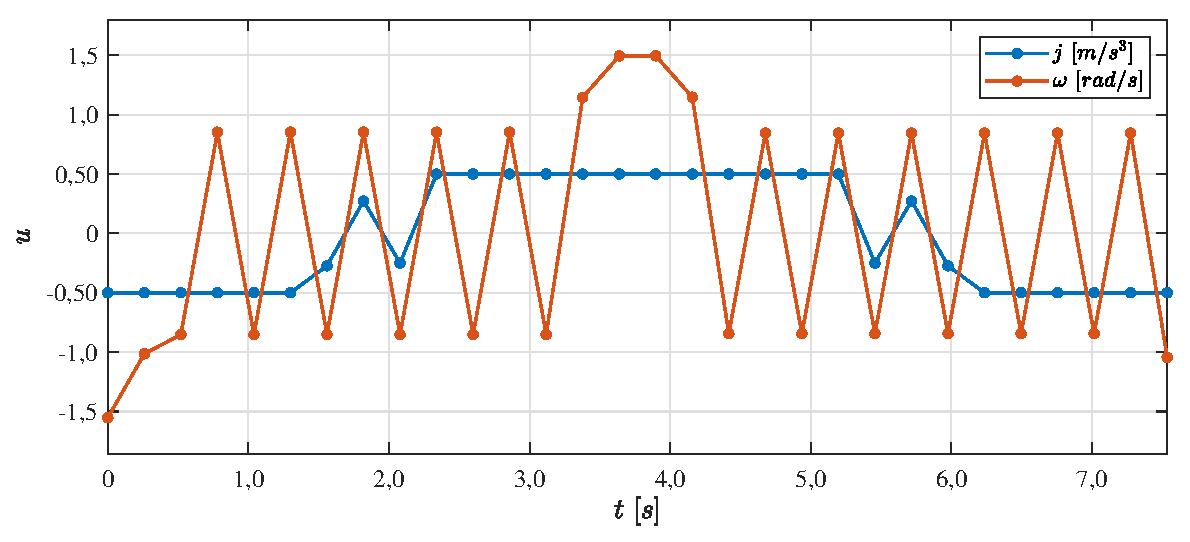
\includegraphics[width=1\linewidth]{fig/resultados/obs/J=u2/estacionamento}
	\captionof{figure}[Trajetórias de controle obtidas pelo emprego do $ PSOPT_t $ na resolução do problema do estacionamento]{Trajetórias de controle obtidas pelo emprego do $ PSOPT_t $ na resolução do estudo de caso introduzido na Seção \ref{sec:resultados:estacionamento}.}
	\label{fig:resultados:conclusao:estacionamento}
	\vspace{\onelineskip}
\end{minipage}

\noindent	
\begin{minipage}{\textwidth}
	\vspace{\onelineskip}
	\centering
	\includegraphics[width=1\linewidth]{fig/resultados/obs/J=u2/estacionamentoJ=u2}
	\captionof{figure}[Suavização das trajetórias de controle obtidas pelo emprego do $ PSOPT_t $ na resolução do problema do estacionamento]{Trajetórias de controle obtidas pelo emprego do $ PSOPT_t $ na resolução do estudo de caso introduzido na Seção \ref{sec:resultados:estacionamento}, considerando-se a definição de uma nova função objetivo $ J' $ segundo \eqref{eq:resultados:conclusao:Jlinha}.}
	\label{fig:resultados:conclusao:estacionamentoJ=u2}
	\vspace{\onelineskip}
\end{minipage}

Na Figura \ref{fig:resultados:conclusao:singular2} são apresentadas as trajetórias de controle obtidas pelo emprego do $ COPILOTS_t $ na resolução do estudo de caso introduzido na Seção \ref{sec:resultados:estacionamento}, adotando-se $ N = 30 $. A trajetória em azul é obtida considerando-se a função objetivo original, enquanto a obtenção daquela em vermelho é baseada na definição uma nova função objetivo $ J' $ definida segundo \eqref{eq:resultados:conclusao:Jlinha}. Comparando-se essas trajetórias, fica claro mais uma vez que a definição de $ J' $ possibilita a obtenção de trajetórias mais suaves. 

\noindent	
\begin{minipage}{\textwidth}
	\vspace{\onelineskip}
	\centering
	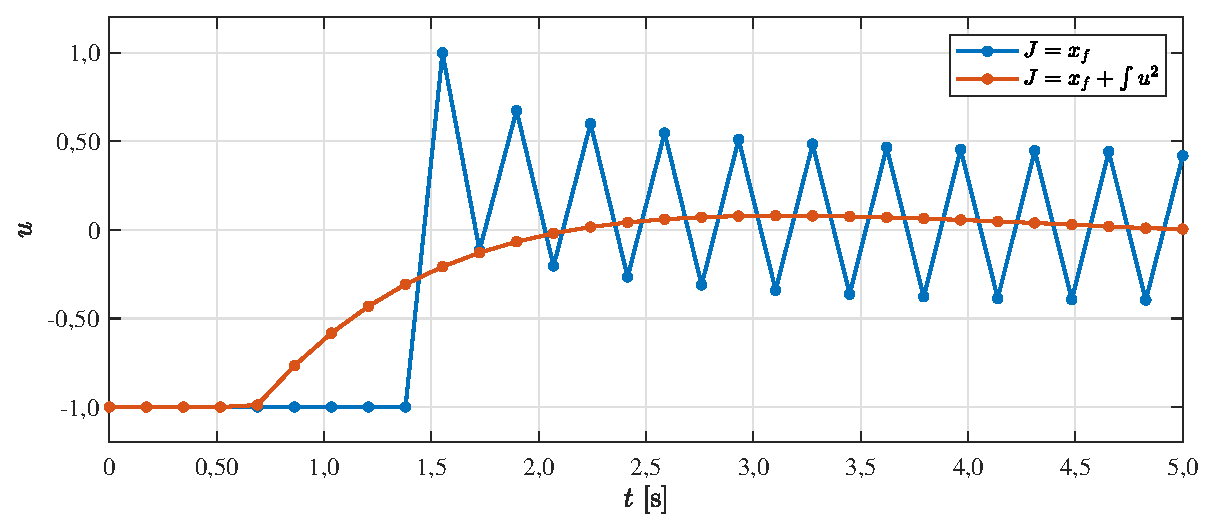
\includegraphics[width=1\linewidth]{fig/resultados/obs/J=u2/singular2}
	\captionof{figure}[Suavização das trajetórias de controle obtidas pelo emprego do $ PSOPT_t $ na resolução do problema singular 2]{Comparação entre a trajetória de controle associadas ao $ PSOPT_t $, introduzida na Seção \ref{sec:resultados:singular2}, e aquela obtida a partir da resolução do estudo de caso introduzido nessa seção definindo-se uma nova função objetivo $ J' $ segundo \eqref{eq:resultados:conclusao:Jlinha}.}
	\label{fig:resultados:conclusao:singular2}
	\vspace{\onelineskip}
\end{minipage}

A definição de uma nova função objetivo $ J' $ segundo \eqref{eq:resultados:conclusao:Jlinha} pode ser considerada inclusive na resolução de PCOs singulares, uma vez que, mesmo quando o PCO ao qual atribui-se $ J $ é singular, o PCO formulado a partir da definição de $ J' $ não o será \cite{jacobson_computation_1970}. No entanto, é preciso ressaltar que a definição de uma nova função objetivo pode ocasionar a deterioração da solução obtida. Por exemplo, no caso do PCO introduzido na Seção \ref{sec:resultados:estacionamento}, Figuras \ref{fig:resultados:conclusao:estacionamento} e \ref{fig:resultados:conclusao:estacionamentoJ=u2}, obtém-se $ t_f = 7,35$ s considerando-se a função objetivo original, enquanto que adotando-se $ J' $, tem-se $ t_f = 7,98 $ s.



